% Also note that the "draftcls" or "draftclsnofoot", not "draft", option
% should be used if it is desired that the figures are to be displayed in
% draft mode.
%
\documentclass[conference]{IEEEtran}
% Add the compsoc option for Computer Society conferences.

% Some very useful LaTeX packages include:
% (uncomment the ones you want to load)

\usepackage{cite}
\ifCLASSINFOpdf
   \usepackage[pdftex]{graphicx}
  % declare the path(s) where your graphic files are
   \graphicspath{{Images/}}
  % and their extensions so you won't have to specify these with
  % every instance of \includegraphics
   \DeclareGraphicsExtensions{.pdf,.jpeg,.png}
\else
  % or other class option (dvipsone, dvipdf, if not using dvips). graphicx
  % will default to the driver specified in the system graphics.cfg if no
  % driver is specified.
  % \usepackage[dvips]{graphicx}
  % declare the path(s) where your graphic files are
  % \graphicspath{{../eps/}}
  % and their extensions so you won't have to specify these with
  % every instance of \includegraphics
  % \DeclareGraphicsExtensions{.eps}
\fi
% graphicx was written by David Carlisle and Sebastian Rahtz. It is
% required if you want graphics, photos, etc. graphicx.sty is already
% installed on most LaTeX systems. The latest version and documentation
% can be obtained at: 
% http://www.ctan.org/tex-archive/macros/latex/required/graphics/
% Another good source of documentation is "Using Imported Graphics in
% LaTeX2e" by Keith Reckdahl which can be found at:
% http://www.ctan.org/tex-archive/info/epslatex/
%
% latex, and pdflatex in dvi mode, support graphics in encapsulated
% postscript (.eps) format. pdflatex in pdf mode supports graphics
% in .pdf, .jpeg, .png and .mps (metapost) formats. Users should ensure
% that all non-photo figures use a vector format (.eps, .pdf, .mps) and
% not a bitmapped formats (.jpeg, .png). IEEE frowns on bitmapped formats
% which can result in "jaggedy"/blurry rendering of lines and letters as
% well as large increases in file sizes.
%
% You can find documentation about the pdfTeX application at:
% http://www.tug.org/applications/pdftex


% correct bad hyphenation here
\hyphenation{op-tical net-works semi-conduc-tor}

\usepackage{url}

\begin{document}
%
% paper title
% can use linebreaks \\ within to get better formatting as desired
% Do not put math or special symbols in the title.
\title{iTrust Interviews}


% author names and affiliations
% use a multiple column layout for up to three different
% affiliations
\author{\IEEEauthorblockN{Justin Smith, Brittany Johnson, and Emerson Murphy-Hill}
\IEEEauthorblockA{North Carolina State University\\
Raleigh, North Carolina}}


% conference papers do not typically use \thanks and this command
% is locked out in conference mode. If really needed, such as for
% the acknowledgment of grants, issue a \IEEEoverridecommandlockouts
% after \documentclass

\maketitle

% As a general rule, do not put math, special symbols or citations
% in the abstract
\begin{abstract}

Assuring the security of software systems requires input from precise and discerning developers.
To assist in this process, new tools and approaches should help answer the security-relevant questions that developers would otherwise struggle with. 
To understand the knowledge requirements of 
To assist developers in this process we must first understand their knowledge requirements.
To enhance our understanding, we conducted 10 semi-structured interviews with software developers, observing their interactions with security vulnerabilities. 
From these interactions, we extracted questions developers asked while assessing the security of iTrust, a Java medical records software system. 
Participants asked X questions which we grouped into Y categories. RESULTS...
Tool IMPLICATIONS...

Educators?

What topic?

\end{abstract}

% no keywords

% For peer review papers, you can put extra information on the cover
% page as needed:
% \ifCLASSOPTIONpeerreview
% \begin{center} \bfseries EDICS Category: 3-BBND \end{center}
% \fi
%
% For peerreview papers, this IEEEtran command inserts a page break and
% creates the second title. It will be ignored for other modes.
\IEEEpeerreviewmaketitle



\section{Introduction}
% no \IEEEPARstart
General Problem

Widespread security vulnerabilities enable potential attackers to exploit vital software systems. 
Distributing a defective piece of software may compromise the security of the entire system. 
Accordingly, research and industry increasingly stress the importance of identifying and eliminating  vulnerabilities as early as possible in their systems~\cite{austin2011one, bessey2010few}. 
When analyzing source code, especially defective code, research suggests that during this knowledge acquisition process, developers hypothesize about the code, specifically by asking questions ~\cite{latoza2010hard, ko2004designing}. 
This area of research also suggests that there may be a need for tool support to help developers answer the questions they have about their code~\cite{latoza2010hard}. 

There exists a variety of tools and techniques developed to assist developers with writing and analyzing code, however, often developers do not use these tools~\cite{}.

Related Stuff

Developers are concerned with the security of their applications, but lack adequate support for reasoning about the security of their systems [CITE?].
Toolsmiths are equipped with an exhaustive set of research findings and guidelines to aid in the design of usable tools [CITE]. 
However, their tools go unused, in part because they do not help developers answer relevant questions or find relevant information~\cite{johnson2013don, latoza2010hard}. 
In fact, research suggests that some of the hard to answer questions developers have pertain to the security of their code~\cite{latoza2010hard}. There exists research that determines the questions developers ask about their code. 
However, to our knowledge, there does not exist research that explores the questions developers ask specifically pertaining to security vulnerabilities in their code. 
Our work aims to inform toolsmiths of the security-related questions that developers ask by assessing knowledge requirements developers have when understanding potential security vulnerabilities.


What is the paper about
	What did we do

In this paper, we report a study conducted with 10 developers familiar with the iTrust software system.~\footnote{\url{http://agile.csc.ncsu.edu/iTrust/wiki/doku.php?id=start}} We observed each developer as they assessed potential security vulnerabilities in the code and report the kinds of questions they asked while doing so. Using a card sort methodology, we sorted XXX cards into XXX categories. [QUICK SUMMARY OF FINDINGS]. 

Contribution

The main contribution of this paper is categorized questions developers ask to inform toolsmiths of knowledge requirements developers have when faced with security vulnerabilities.

The remainder of the paper is organized as follows. In Section~\ref{sec:rw}, we discuss previous work related to our own. Section~\ref{sec:meth} outlines the methodology we used to conduct our study and analyze our data. Next, we discuss the findings of our study in Section~\ref{sec:results} and implications of our findings in Section~\ref{sec:disc}. Finally, we conclude the paper with a discussion of future work~\ref{sec:fw}.



% An example of a floating figure using the graphicx package.
% Note that \label must occur AFTER (or within) \caption.
% For figures, \caption should occur after the \includegraphics.
% Note that IEEEtran v1.7 and later has special internal code that
% is designed to preserve the operation of \label within \caption
% even when the captionsoff option is in effect. However, because
% of issues like this, it may be the safest practice to put all your
% \label just after \caption rather than within \caption{}.
%
% Reminder: the "draftcls" or "draftclsnofoot", not "draft", class
% option should be used if it is desired that the figures are to be
% displayed while in draft mode.
%
%\begin{figure}[!t]
%\centering
%\includegraphics[width=2.5in]{myfigure}
% where an .eps filename suffix will be assumed under latex, 
% and a .pdf suffix will be assumed for pdflatex; or what has been declared
% via \DeclareGraphicsExtensions.
%\caption{Simulation Results.}
%\label{fig_sim}
%\end{figure}

% Note that IEEE typically puts floats only at the top, even when this
% results in a large percentage of a column being occupied by floats.


% An example of a double column floating figure using two subfigures.
% (The subfig.sty package must be loaded for this to work.)
% The subfigure \label commands are set within each subfloat command,
% and the \label for the overall figure must come after \caption.
% \hfil is used as a separator to get equal spacing.
% Watch out that the combined width of all the subfigures on a 
% line do not exceed the text width or a line break will occur.
%
%\begin{figure*}[!t]
%\centering
%\subfloat[Case I]{\includegraphics[width=2.5in]{box}%
%\label{fig_first_case}}
%\hfil
%\subfloat[Case II]{\includegraphics[width=2.5in]{box}%
%\label{fig_second_case}}
%\caption{Simulation results.}
%\label{fig_sim}
%\end{figure*}
%
% Note that often IEEE papers with subfigures do not employ subfigure
% captions (using the optional argument to \subfloat[]), but instead will
% reference/describe all of them (a), (b), etc., within the main caption.


% An example of a floating table. Note that, for IEEE style tables, the 
% \caption command should come BEFORE the table. Table text will default to
% \footnotesize as IEEE normally uses this smaller font for tables.
% The \label must come after \caption as always.
%
%\begin{table}[!t]
%% increase table row spacing, adjust to taste
%\renewcommand{\arraystretch}{1.3}
% if using array.sty, it might be a good idea to tweak the value of
% \extrarowheight as needed to properly center the text within the cells
%\caption{An Example of a Table}
%\label{table_example}
%\centering
%% Some packages, such as MDW tools, offer better commands for making tables
%% than the plain LaTeX2e tabular which is used here.
%\begin{tabular}{|c||c|}
%\hline
%One & Two\\
%\hline
%Three & Four\\
%\hline
%\end{tabular}
%\end{table}


%Figure, high res, png or vector (pdf)

\section{Related Work}
\label{sec:rw}

We have organized the related work into three sections. Section \ref{evaluation} outlines the predominant approaches researchers use to evaluate security tools. Section \ref{understanding} surveys the work done to facilitate developers' understanding of code, and section \ref{questions} references similar studies that have explored the questions developers ask when modifying, understanding, or debugging their code.

\subsection{Evaluation of Techniques}
\label{evaluation}
Developers use several techniques and tools to help secure their systems.
Using a variety of metrics, many studies have assessed the effectiveness of the tools and techniques developers use to find and remove vulnerabilities from their code~\cite{martin2005finding, austin2011one, livshits2005finding}.  

Much research has evaluated the effectiveness of tools and techniques based on their false positive rates and how many vulnerabilities they detect~\cite{jovanovic2006pixy, austin2011one, dukes2013case}. 
Jovanovic and colleagues attempt to address the problem of vulnerabilities in web applications by implementing and evaluating \textsc{Pixy}, a static analysis tool that detects cross-site scripting vulnerabilities in PHP scripts~\cite{jovanovic2006pixy}. 
They considered their tool effective because of its low false positive rate (50\%) and its ability to find vulnerabilities previously unknown. 
Similarly, Livshits and Lam evaluated their own approach to static analysis for detecting security vulnerabilities; the static analyzers used are created from specifications provided by the user~\cite{livshits2005finding}. 
They also found their tool to be effective because it had a low false positive rate. 

Austin and Williams compared the effectiveness of four existing techniques for discovering security vulnerabilities: systematic and exploratory manual  penetration testing, static analysis, and automated penetration testing~\cite{austin2011one}. 
Comparing the four approaches based on number of vulnerabilities found, false positive rate, and efficiency, they reported that no one technique was capable of discovering every type of vulnerability. 
Dukes and colleagues conducted a case study comparing static analysis and manual testing techniques used to find security vulnerabilities~\cite{dukes2013case}. 
They found that the combination of manual testing and static analysis was most effective, because it found the most vulnerabilities.


These studies use various measures of effectiveness, such as false positive rates or vulnerabilities found by a tool, but none focus on how developers interact with the tool. Further, they do not evaluate whether the tools under study answer questions that developer have about the code or vulnerabilities. 
Unlike existing studies, our study explores the questions developers ask when attempting to understand the vulnerabilities in their code.

\subsection{Developer Understanding}
\label{understanding}
In other, non-security domains, research has shifted focus from the technical effectiveness of program analysis tools to usability~\cite{johnson2013don, ayewah2008using, khoo2008path}. 
These studies sought to evaluate how tools communicate information to developers and how a tool can enhance a developer's understanding of the code. Such studies examine proposed and existing approaches using various qualitative methods such as interviews and surveys. 

Some research surrounding tool effectiveness shifted focus from technical effectiveness of program analysis tools to usability~\cite{johnson2013don, ayewah2008using, khoo2008path}. The goal of these studies was to evaluate how tool designers can help developers cope with existing or proposed approaches, through comparison of proposed and existing approaches and various qualitative methods, such as interviews and surveys.

Ayewah, Pugh, and colleagues conducted a series of interviews and surveys, along with a controlled user study, in an attempt to better understand the practices and needs of developers when using the static analysis tool FindBugs~\cite{ayewah2008report, ayewah2008using}.

Khoo and colleagues focused their efforts on improving the user interface of existing tools by developing and evaluating \textsc{Path Projection}, a user interface toolkit to help developers navigate through and understand the errors in their code~\cite{khoo2008path}.

Johnson and colleagues conducted semi-structured interviews with professional developers to determine the reason developers have for using, and possibly not using, static analysis tools to find defects in their codes~\cite{johnson2013don}. 
Their findings suggest that one of the biggest reasons developers may have for not using tools to analyze their code is difficulty understanding the output provided. 

Layman and colleagues conducted a study with developers to explore the factors developers consider when deciding whether they will fix a defect or not~\cite{layman2007toward}. Based on their findings, they discuss design implications for automated fault detection tools.

These studies discuss the ability of developers to effectively use existing tools and ways to improve them, however, they do not pay due diligence to how developers interpret the reporting of security vulnerabilities. 
It is particularly important to consider security tools and vulnerabilities, because security vulnerabilities are more likely to cause incidents that affect company budgets as well as the end users~\cite{chen2002mops}. 
Research also suggests that some of the harder questions to answer when analyzing code revolve around security and the implications of changes made to the code on security~\cite{latoza2010hard}.  
The goal of our study is to identify the security-related questions developers ask when approaching security vulnerabilities so that tool designers understand the information requirements of security-minded developers.

\subsection{Answering Developer Questions}
\label{questions}
Several studies have explored the knowledge requirements of developers, however few such studies have focused specifically on the knowledge requirements of developers when assessing security vulnerabilities~\cite{begel2014analyze, latoza2010hard, latoza2010developers}.

LaToza and Myers surveyed professional software developers to understand the questions developers ask during their daily coding activities, focusing on the hard to answer questions~\cite{latoza2010hard}. 

Futhermore, after observing developers in a lab study, they discovered that the questions developers ask tend to be questions revolving around searching through the code for target statements, or reachability questions~\cite{latoza2010developers}. 

Ko and Myers developed \textsc{Whyline}, a tool meant to ease the process of debugging code by helping answer ``why did'' and ``why didn't'' questions developers have~\cite{ko2004designing}. They found that developers were able to complete more debugging tasks when using their tool than they could without it.

Fritz and Murphy developed a model and prototype tool to assist developers with answering the questions they want to ask based on interviews they conducted~\cite{fritz2010using}.

%we know finding answers tedious; our study aims to find the questions and ways tool designers can help developers with this process.  

These studies explore the questions developers ask when building and debugging software, however, they do not study the questions developers ask when they have a potential security vulnerability in their code. 
In fact, our work builds on the work of LaToza and Myers, which found that some of the hard-to-answer questions developers have pertain to the implications of code changes on the security of their code. 
Our study aims to discover the questions developers have about potential code vulnerabilities and the implications of the changes they may make when attempting to resolve them. 

\section{Methodology}
\label{sec:meth}
We conducted 10 semi-structured interviews with software developers. In our analysis, we extracted and categorized the questions developers asked during these interviews. Section \ref{rqs} outlines the research questions we sought to answer. Section \ref{studyDesign} details how the study was designed and section \ref{dataAnalysis} describes how we preformed data analysis.


\subsection{Research Questions}
\label{rqs}
We want to answer the following research questions:
\begin{itemize}
\item \textbf{RQ1}: What types of security related questions do developers ask?
\item \textbf{RQ2}: What types of security related questions do developers fail to answer?
\end{itemize}

\subsection{Study Design}
\label{studyDesign}
Each interview started with a five-minute briefing section, followed by encounters with four vulnerabilities.
All participants consented to have their session recorded using screen and audio capture software.
Finally, each interview concluded with several demographic and open-ended discussion questions.


\subsubsection{Materials}

\begin{figure}
\centering
\includegraphics[width=3in]{Images/environment.png}
\caption{The environment participants were presented with.}
\label{fig:environment} 
\end{figure}
	

Participants used Eclipse to explore vulnerabilities in iTrust,\footnote{\url{agile.csc.ncsu.edu/iTrust/wiki/doku.php}} a Java medical records application that ensures the privacy and security of patient records according to the HIPAA statue.\footnote{\url{hhs.gov/ocr/privacy/}} 
During the briefing session, participants were given time to familiarize themselves with the development environment and ask any questions about the experimental setup.
Participants were equipped with an extended version FindBugs, Find Security Bugs.\footnote{\url{http://h3xstream.github.io/find-sec-bugs/}} 
We chose Find Security Bugs as a representative tool by comparing the available source code analysis tools listed by NIST, OWASP, and WASC. Figure \ref{fig:environment} depicts the configuration of the IDE for one of the tasks.


\subsubsection{Participants}
We interviewed a total of 10 software developers, 6 students and 4 professionals. 
All interviews were conducted in-person.
We recruited participants from personal contacts and class rosters, using snowball sampling to find additional qualified participants.
Since extracting data from each interview required intensive analysis, we ceased recruitment when we felt that few new questions were emerging from each additional interview.
To simulate a more realistic work environment, participants were required to have significant experience working on the iTrust code base. All participants either completed or served as teaching assistants for a semester-long software engineering course that focused on developing iTrust.
Table ?? gives additional demographic information on each of the 10 participants. 
WHY DEMOGRAPHIC INFO? ensure a degree of diversity in our sample. Cross group analysis??

\subsubsection{Tasks}
Each participant approached four vulnerabilities. We presented each participant with this number of vulnerabilities, because in preliminary pilot interviews, participants spent approximately 10-15 minutes with each vulnerability and showed signs of fatigue after 60 minutes.

FindBugs and Find Security Bugs group similar error messages using a system of tags. For example the Null Pointer tag (NP) applies to notifications that warn about the misuse of null. To cover a broader set of question topics, we selected vulnerabilities with four different tags.
Find Security Bugs identified three types of naturally occurring vulnerabilities: cross site scripting, path traversal, and predictable random vulnerabilities.
We inserted a SQL injection vulnerability by making minimal modifications to one of the database access objects.
Our modifications preserved the functionality of the original code and were based on examples of SQL injection presented by OWASP.
Table xx summarizes each of the four vulnerabilities. 

During the briefing section, participants were told that they were in charge of security for iTrust and to approach the vulnerabilities as if they were in their normal work environment.
Additionally, we asked them to use a think aloud protocol. Specifically, they were asked to, "Say any questions or thoughts that cross your mind regardless of how relevant you think they are."

The interviewer was equipped with the following script, but had the freedom to omit questions or ask follow-up questions based on the participant's responses.
\begin{itemize}
\item What are you exploring/trying to figure out right now?
\item What information do you need to proceed?
\item Can you explain what this warning is trying to tell you?
\item Based on your understanding of this error message, what is the percentage likelihood you would modify this section of he code?
\item How would you fix the problem? Where would you start?
\item On a scale of 1-5, how confident are you in your understanding of the error message?
\item On a scale of 1-5, how confident are you that you are making the correct judgments?
\item What information would you like to see added to the error message?
\item What part of the message is most helpful?
\item Look at the error message one last time. Is there any information you initially disregarded?
\item Is there anything else that you think I should know about this vulnerability?

\end{itemize}

\subsection{Data Analysis}
\label{dataAnalysis}
What is grounded theory [CITE]. 

First, we transcribed all the audio files using oTranscribe.\footnote{\url{otranscribe.com}}
Using a grounded theory approach, each of the interviews was analyzed by two of the authors for implicit and explicit questions. 
We also extracted demographic information, self-efficacy scores and whether or not the participant would modify the code. ?? The two question sets for each interview were then iteratively compared against each other until the authors reached agreement on the question sets. 
In the remainder of this section, we will detail the question extraction process and question sorting processes, including the criteria used to determine which statements qualified as questions.
\subsubsection{Question Criteria}
[CITE LETOVSKY] HERE

Participants ask both explicit and implicit questions. We developed 5 criteria to assist in the uniform classification of participant statements. A statement was coded as a question only if it met one of the following criteria:

\begin{itemize}
\item \textbf{The participant explicitly asks a question.}
\\ P2: \textit{Why aren't they using Prepared Statements?}
\item \textbf{The participant makes a statement and explores the validity of that statement.}
\\ P6: \textit{It doesn't seem to have shown what I was looking for. Oh, wait! It's right above it...}
\item \textbf{The participant uses key words such as, "I assume," "I guess," or "I don't know."}
\\ P8: \textit{I don't know that it's a problem yet.}
\item \textbf{The participant clearly expresses uncertainty over a statement.}
\\ P10: \textit{Well, it's private to this object, right?}
\item \textbf{The participant clearly expresses a knowledge requirement by describing plans to acquire information.}
\\ P1: \textit{I would figure out where it is being called.}

\end{itemize}

\subsubsection{Question Extraction}
Using the criteria outlined in the previous section, each interview was independently coded for questions by two of the authors. 
When we identified a statement that satisfied one or more of the criteria, we marked the transcript, highlighting the participants original statement, and clarified the question being asked.

%Include the figure here!
FIGURE OF WORD


To handle instances where the two coders disagreed, each interview was reviewed a second time by the two authors that initially coded it.
During the second review, the two reviewers examined each question statement, discussing the justification for each question based on the previously stated criteria.
If one of the reviewers did not agree that a question met at least one of the criteria, the question was removed from the question set. 
When reviewers did agree, they determined the phrasing for the question that was most strongly grounded in the interview artifacts. 
Depending on the participant, inter-reviewer agreement ranged from 91\% to 100\%. Across all participants, agreement averaged to 95\%.

\subsubsection{Question Sorting}
To organize our questions and facilitate discussion, we preformed an \textit{open} card sort~\cite{hudson2013sorting}. 
Card sorting is typically used to help structure data by grouping related information into categories. 
In an \textit{open} sort, the process begins with no notion of predefined categories. 
Rather, sorters derive categories from emergent themes in the cards. 

%\begin{figure}
%\centering
%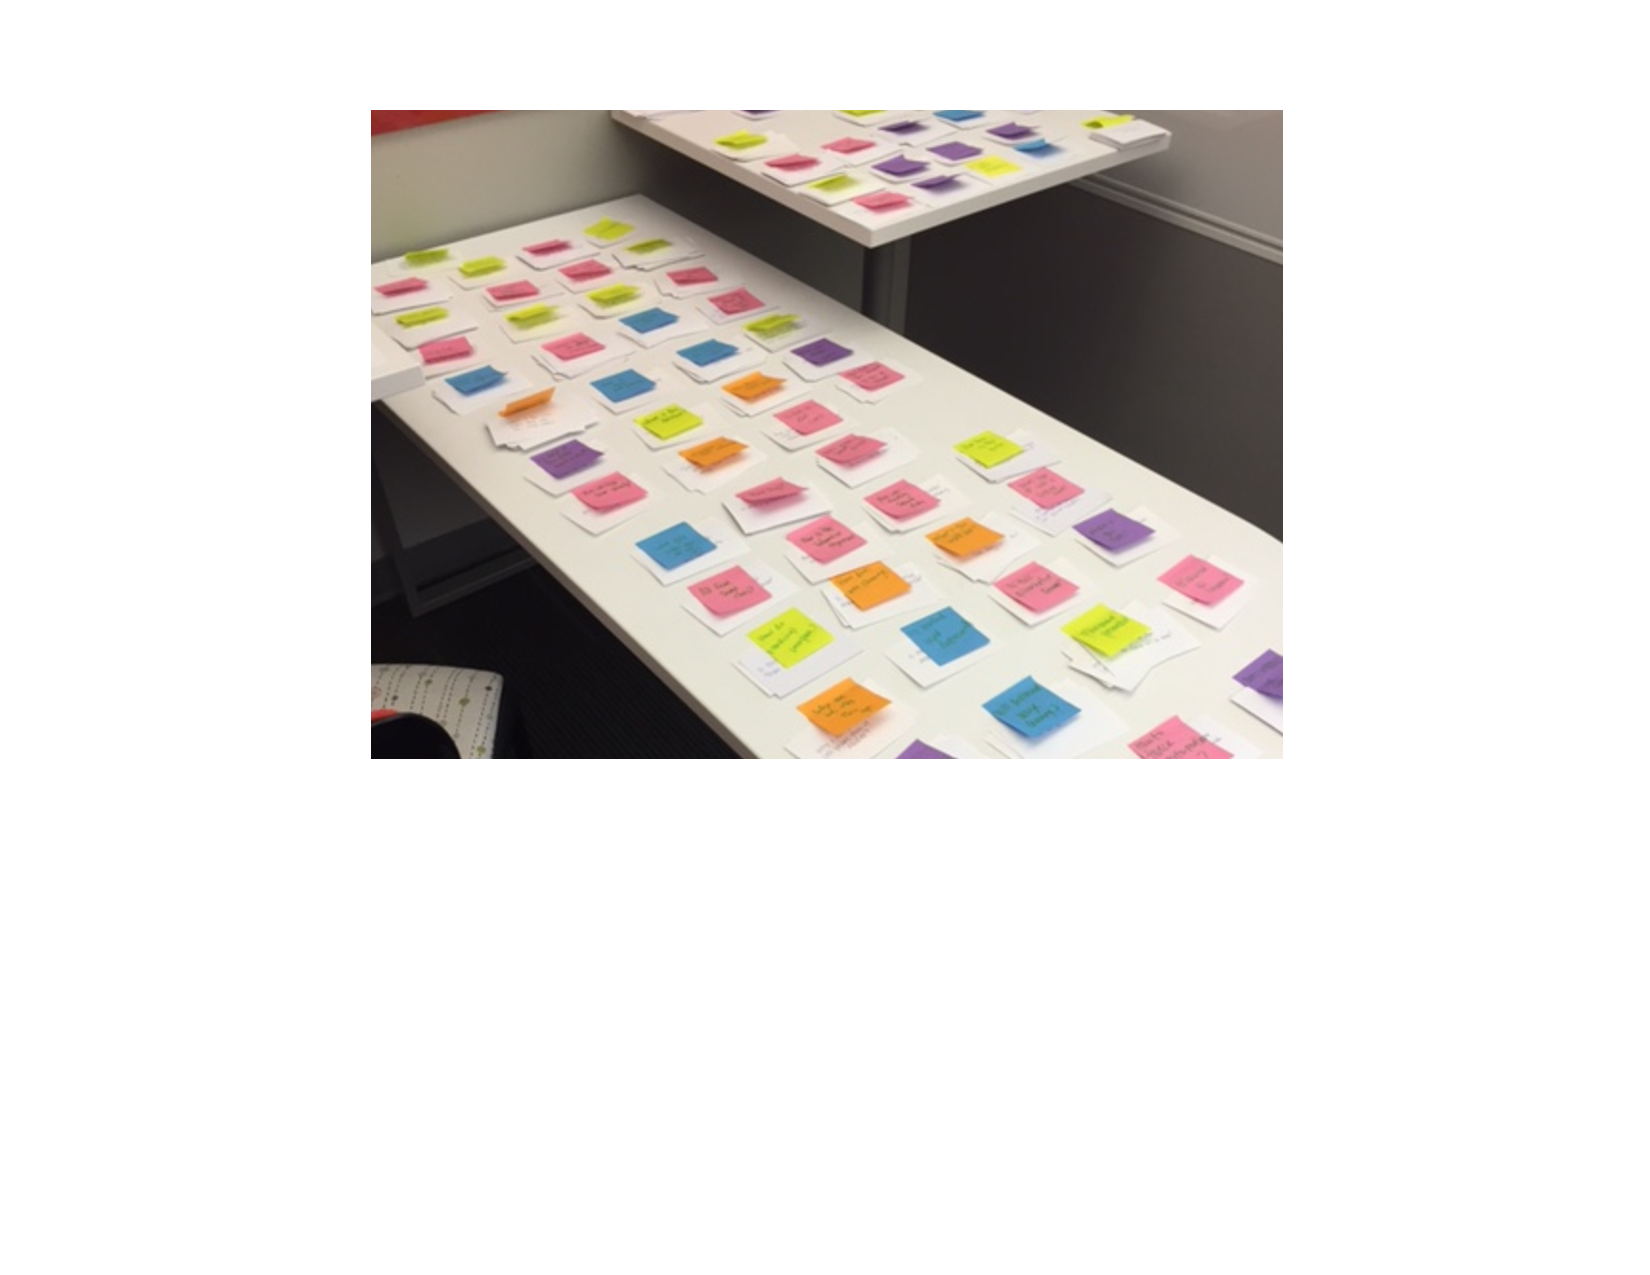
\includegraphics[width=3in]{Images/notecards.pdf}
%\caption{Result of initial card sorting.}
\label{fig:cardsort} 
%\end{figure}

We preformed our card sort in three stages. 
In the first stage we formed question clusters by grouping questions that identified the same information requirements (Figure~\ref{fig:cardsort}). 
For example, (EXAMPLES)

%\begin{figure}
%\centering
%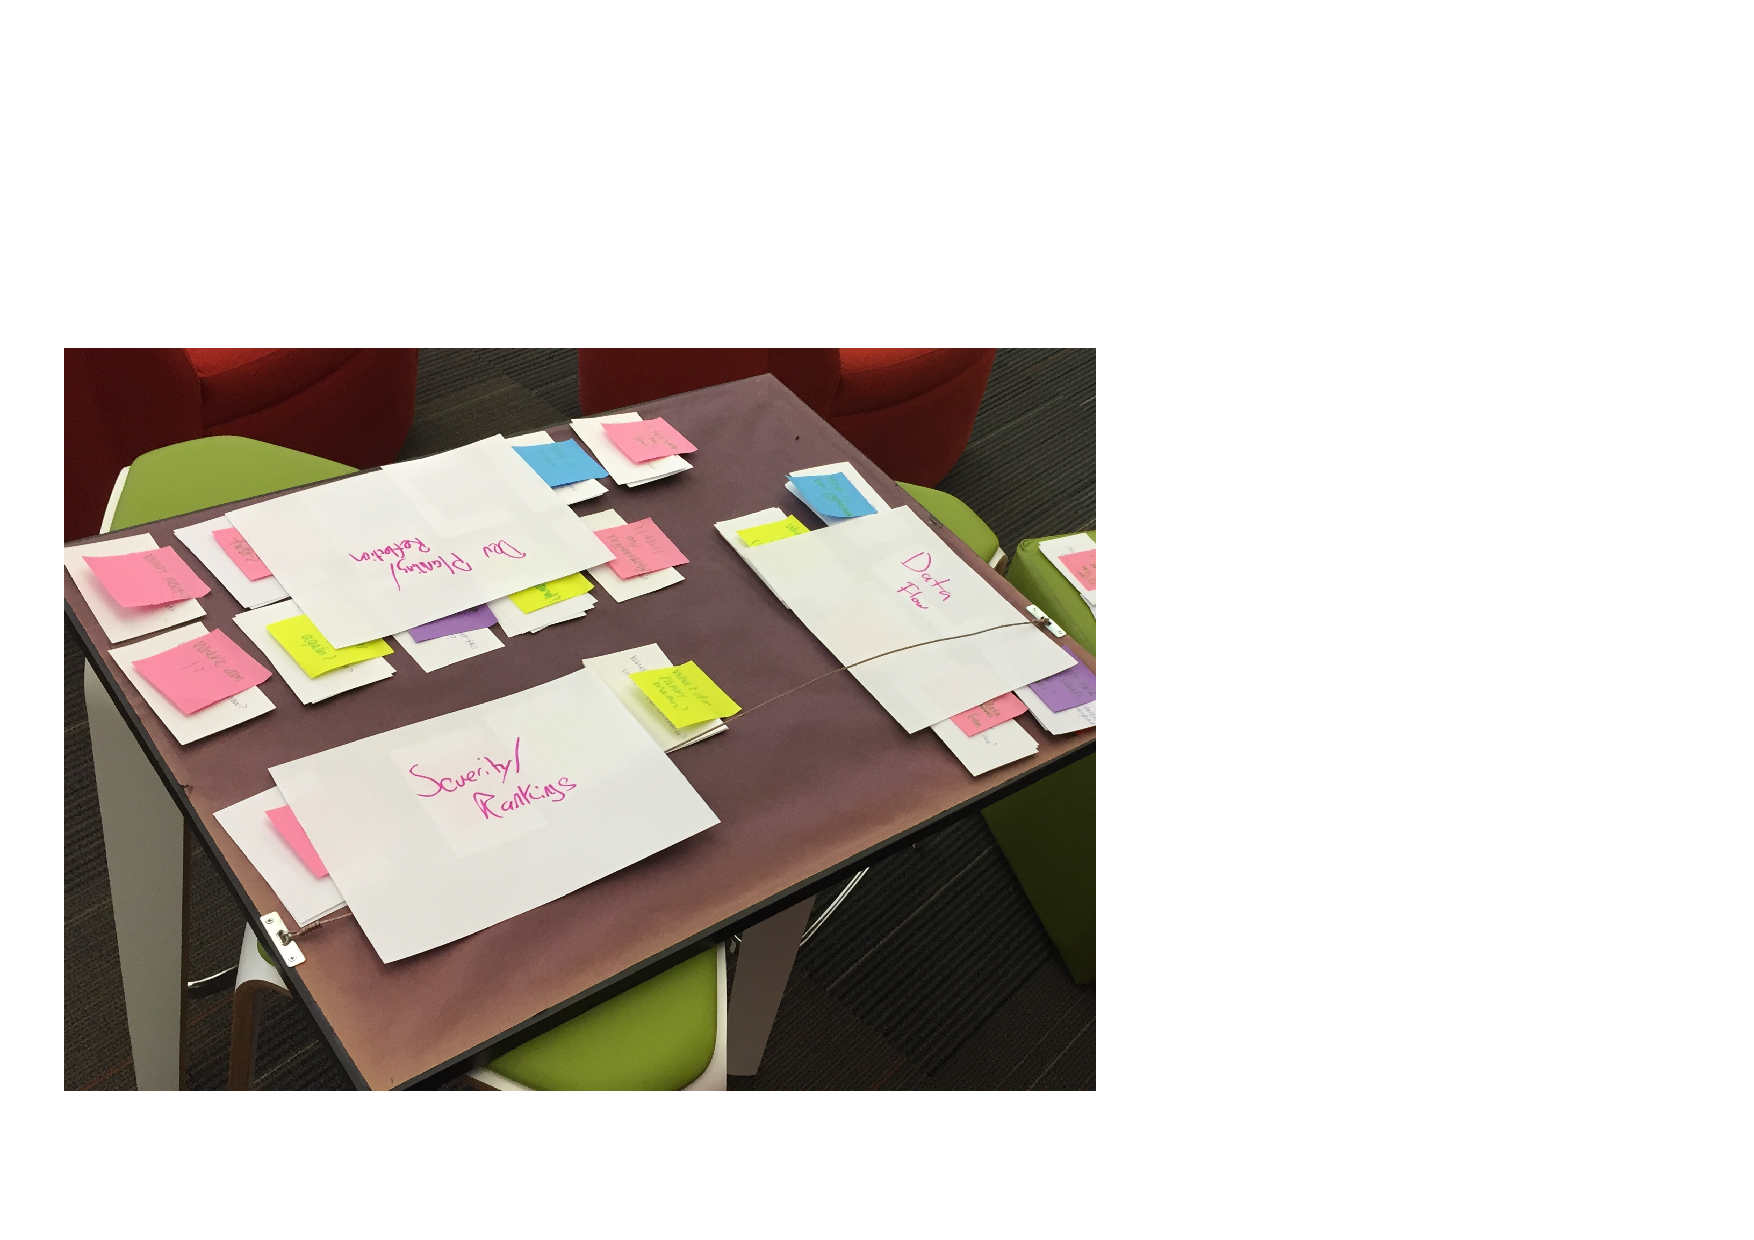
\includegraphics[width=3in]{Images/categories.pdf}
%\caption{Sorting cards into categories based on emergent themes.}
%\label{fig:cardsort} 
%\end{figure}

In the second stage we identified emergent themes and grouped the clusters into categories based on the themes. 
Table ?? contains the X categories along with the number of distinct clusters each contains.

To validate the categories we identified, DESCRIBE VERIFICATION STAGE! 

-Card Sorting
Dr. E Category validation?


\section{Results}
\label{sec:results}
We extracted x questions, removing repeats, we came up with x questions

Following the most similar work to our own, for each category, we list each distinct question we extracted and the count for each in parenthesis~\cite{latoza2010hard}. We also discuss the common thread between the questions in each category and speculate as to why these bits of information may be important when assessing potential security vulnerabilities.

\noindent\subsection{\textbf{Developer Planning and Self-Reflection (11)}} 

\noindent\emph{What was I looking for?} \\
\emph{What do I know now?} \\
\emph{What should I do first?} \\
\emph{Do I understand?} \\
\emph{Have I seen this before?} \\
\emph{What was that again?} \\
\emph{What's next?} \\
\emph{Where am I in the code?} \\
\emph{Is this worth my time?} \\
\emph{Is this my responsibility?} \\
\emph{Why do I care?} \\
\emph{Miscellaneous} \\

One kind of question participants asked when assessing potential security vulnerabilities in the code concerned their current status or plans for next steps in terms of understanding or assessing the vulnerability. Nine of the XXX distinct questions extracted fit into this category. All of the questions in this category involve general thoughts the developer has pertaining to the vulnerability, rather than specifics of the code or the error notification.  The most common occurring question in this category was...

Though these general questions may not be trivial to help developers answer, there may be ways to provide information or instructions developers can follow to more easily determine the answers for themselves. For example, one question participants asked was ``Have I seen this before?'' A tool that helps developers answer this question might keep track of previous times the developer has encountered, and perhaps fixed, this vulnerability. The tool could also include a link to the code where the vulnerability was located as well as a diff showing the changes the developer made to fix the vulnerability.

%%%%%%%%%%%% Code Background

\noindent\subsection{\textbf{Code Background and Function (9)}}

\noindent\emph{Who wrote this code?} \\
\emph{Why is this code needed?} \\
\emph{Is this library code??} \\
\emph{Are there tests for this code?} \\
\emph{Why was this code written this way?} \\
\emph{What does this code do?} \\
\emph{Is this code doing anything?} \\
\emph{How much effort was put into this code?} \\
\emph{Why are we using this API in the code?} \\
\emph{Miscellaneous} \\

Another kind of question participants asked concerned the background and intended function of the code being analyzed. Nine of the XXX distinct questions extracted fit into this category. The questions in this category aim to learn more about the code at an abstract level, such as determining the role a component or piece of code plays in the entire system or program.

The answer to many of these questions would require aggregated data, such as documentation that programmers contribute to as the code changes or measuring the amount of effort that has been put into the code thus far...
One example of this would be...


%%%%%%%%%%%% Locating Information

\noindent\subsection{\textbf{Locating Information (9)}}

\noindent\emph{Where is this used in the code?} \\
\emph{Where are other similar pieces of code?} \\
\emph{Where is this artifact?} \\
\emph{Is this artifact located in this class?} \\
\emph{Where is this method defined?} \\
\emph{Where is this class? } \\
\emph{Where is the next occurrence of this variable?} \\
\emph{How do I track this information in the code?} \\
\emph{How do I navigate to other open files?} \\
\emph{Miscellaneous} \\

Some participants asked questions regarding locating, or the ability to locate, various bits of information in their coding environment. Nine questions of the XXX extracted fit into this category. The distinction between this category and \emph{\textbf{Code Background and Function}} is that this category includes questions pertaining to searches made in the coding environment for information, artifacts or code fragments; \emph{\textbf{Code Background and Function}} pertains to understanding the code at a higher level that would not be answered by triaging the code.

The answers to these questions can be found inside the IDE, which makes it more feasible for a tool to attempt to answer it. For example... 


%%%%%%%%%%%% Assessing Application

\noindent\subsection{\textbf{Assessing Application of the Fix (9)}}

\noindent\emph{How hard is it to apply a fix to this code?} \\
\emph{How do I use this fix in my code?} \\
\emph{How do I fix this vulnerability?} \\
\emph{Is there a quick fix for automatically applying a fix?} \\
\emph{Will the code work the same after I apply the fix?} \\
\emph{Can these fix suggestions be applied to my code?} \\
\emph{Will the error go away when I apply this fix?} \\
\emph{Does the code stand up to additional tests prior to/after applying the fix?} \\
\emph{What other changes do I need to make to apply this fix?} \\

Another kind of question participants asked pertained to the process of fixing the code. The goal of these questions were to better understand how they would actually apply a fix to their code and the effects of doing so on their code. 9 of the XXX distinct questions participants asked were put into this category.

Though it is not clear how feasible it is to answer some of these questions, some can be answered by using a similar approach to that used by Mu{\c{s}}lu and colleagues to developer Quick Fix Scout~\cite{mucslu2012speculative}. Their tool attempts to help developers answer the question \emph{does this fix introduce other bugs?} None of our participants asked this question specifically, however, questions like \emph{how hard is it to apply} and \emph{does the code stand to additional tests prior to/after applying} could possibly be answered using a similar process.

  

%%%%%%%%%%%% Preventing and Understanding Potential Attacks 

\noindent\subsection{\textbf{Preventing and Understanding Potential Attacks (9)}}

\noindent\emph{How can this vulnerability lead to an attack?} \\
\emph{How can I replicate an attack that exploits this vulnerability?} \\
\emph{Why is this a vulnerability?} \\
\emph{What are the possible attacks that could occur?} \\
\emph{How can I prevent this attack?} \\
\emph{How should I address this problem? (1)} \\
\emph{What is the problem (potential attack)?} \\
\emph{Is this a real vulnerability?} \\
\emph{How do I find out if this is a real vulnerability?} \\
\emph{Miscellaneous} \\


%%%%%%%%%%%% Data Storage 

\noindent\subsection{\textbf{Data Storage and Flow (8)}}

\noindent\emph{How is data put into this variable?} \\
\emph{Does data from this method/code travel to the database?} \\
\emph{Where does this information/data go?} \\
\emph{How do I find where the information travels?} \\
\emph{How does the information change as it travels through the programs?} \\
\emph{What does the variable contain?} \\
\emph{Is any of the data malicious?} \\
\emph{Where is the data coming from?} \\
\emph{Miscellaneous} \\
\noindent\subsection{\textbf{Bug Severity/Ranking (4)}}

\noindent\emph{How serious is this bug?} \\
\emph{Are all these bugs the same severity?} \\
\emph{How do the rankings compare?} \\
\emph{What do the bug rankings mean?} \\

%%%%%%%%%%%% Control Flow/Call Information

\noindent\subsection{\textbf{Control Flow/Call Information (8)}}

\noindent\emph{What is the call hierarchy?} \\
\emph{How can I get calling information?} \\
\emph{Who can call this?} \\
\emph{Where is the method being called?} \\
\emph{What causes this to be called?} \\
\emph{Are all calls coming from the same class?} \\
\emph{What gets called when this method gets called?} \\
\emph{How often is this code called?} \\
\emph{Miscellaneous} \\


%%%%%%%%%%%% Application Context

\noindent\subsection{\textbf{Application Context/Usage (7)}}

\noindent\emph{What is the method/variable used for in the program?} \\
\emph{Are we handling secure data in this context?} \\
\emph{What is the context of this bug/code?} \\
\emph{How does the system work??} \\
\emph{Will usage of this method change?} \\
\emph{Is the method/variable every being used?} \\
\emph{Is this code used to test the program/functionality?} \\
\emph{Miscellaneous} \\


%%%%%%%%%%%% Resources

\noindent\subsection{\textbf{Resources/Documentation (7)}}

\noindent\emph{What type of information does this resource link me to?} \\
\emph{What is the documentation?} \\
\emph{Can my team members/resources provide me with more information?} \\
\emph{Where can I get more information?} \\
\emph{What information is in the documentation?} \\
\emph{Is this a reliable/trusted resource?} \\
\emph{How do resources prevent or resolve this?} \\
\emph{Miscellaneous} \\


%%%%%%%%%%%% Understanding Interacting Tools

\noindent\subsection{\textbf{Understanding and Interacting with Tools (7)}}

\noindent\emph{Why is the tool complaining?} \\
\emph{What is the tool output telling me?} \\
\emph{Can I verify the information the tool provides?} \\
\emph{What is the tool keybinding?} \\
\emph{What is the tool's confidence?} \\
\emph{What tool do I need for this?} \\
\emph{How is the information presented by the tool organized?} \\
\emph{Miscellaneous} \\



%%%%%%%%%%%% Understanding Alt. Fixes

\noindent\subsection{\textbf{Understanding Alternative Fixes and Approaches (7)}}

\noindent\emph{Why should I use this alternative method/approach to fix the vulnerability?} \\
\emph{What are the alternatives for fixing this?} \\
\emph{Does the alternative function the same as what I'm currently using?} \\
\emph{When should I use the alternative?} \\
\emph{Is the alternative slower?} \\
\emph{Are there other considerations to make when using the alternative(s)?} \\
\emph{How does my code compare to the alternative code in the example I found?} \\
\emph{Miscellaneous} \\



%%%%%%%%%%%% Relationship Between Bugs

\noindent\subsection{\textbf{Relationship Between Bugs (3)}}

\noindent\emph{Does this other piece code have the same bug as the code I'm working with?} \\
\emph{Are all the bugs related in my code?} \\
\emph{Are all of these notifications vulnerabilities?} \\


%%%%%%%%%%%% End-User Interaction

\noindent\subsection{\textbf{End-User Interaction (3)}}

\noindent\emph{Is there input coming from the user?} \\
\emph{Does the user have access to this code?} \\
\emph{Does user input get validated/sanitized?} \\


%%%%%%%%%%%% Error Messages

\noindent\subsection{\textbf{Error Messages (3)}}

\noindent\emph{What is the relationship between the error message and the code?} \\
\emph{What code caused this error message to occur?} \\
\emph{What does the error message say?} \\



%%%%%%%%%%%% Understanding Concepts

\noindent\subsection{\textbf{Understanding Concepts (4)}}

\noindent\emph{What is the term for this concept?} \\
\emph{Do these words have special meaning related to this concept/problem?} \\
\emph{How does this concept work?} \\
\emph{What is this concept?} \\
\emph{Miscellaneous} \\


%%%%%%%%%%%% Confirming Expectations

\noindent\subsection{\textbf{Confirming Expectations (1)}}

\noindent\emph{Is this doing what I expect it to?} \\



\section{Discussion}
\label{sec:disc}
Data suggests that tools should focus on XYZ. Discuss interesting/contradictory categories and implications.

\section{Future Work}
\label{sec:fw}

\section{Conclusion}
\label{sec:concl}
The conclusion goes here.




% conference papers do not normally have an appendix


% use section* for acknowledgement
\section*{Acknowledgment}


The authors would like to thank...


\bibliographystyle{IEEEtran}
% argument is your BibTeX string definitions and bibliography database(s)
\bibliography{iTrustInterviews}
%
% <OR> manually copy in the resultant .bbl file
% set second argument of \begin to the number of references
% (used to reserve space for the reference number labels box)




% that's all folks
\end{document}


